\chapter{Kiến trúc phần Back-end}
\label{Chapter3}
Ở chương này, nhóm sẽ tập trung giải thích về cách thức hoạt động của phần Back-end của hệ thống. Gồm các giai đoạn như sau:
\begin{itemize}
	\item Xử lý dữ liệu thu thập: Mã hoá dữ liệu đã thu thập ở chương 3, lưu trữ dữ liệu vào trong cơ sở dữ liệu.
	\item Xử lý dữ liệu câu hỏi mà người dùng nhập vào trong hệ thống, cách mà hệ thống xử lý câu hỏi của người dùng và đưa ra kết quả cho người dùng.
	

\end{itemize}
\section{Xử lý dữ liệu thu thập}
Trong mục này, xử lý dữ liệu thu thập là tiến hành việc công việc phân loại từ câu hỏi, mã hoá câu hỏi từ dữ liệu bộ câu hỏi và câu trả lời đã thu thập được ở chương 3 và việc lưu trữ dữ liệu xuống Elastic Search.

\begin{figure*}[htp]
\centering
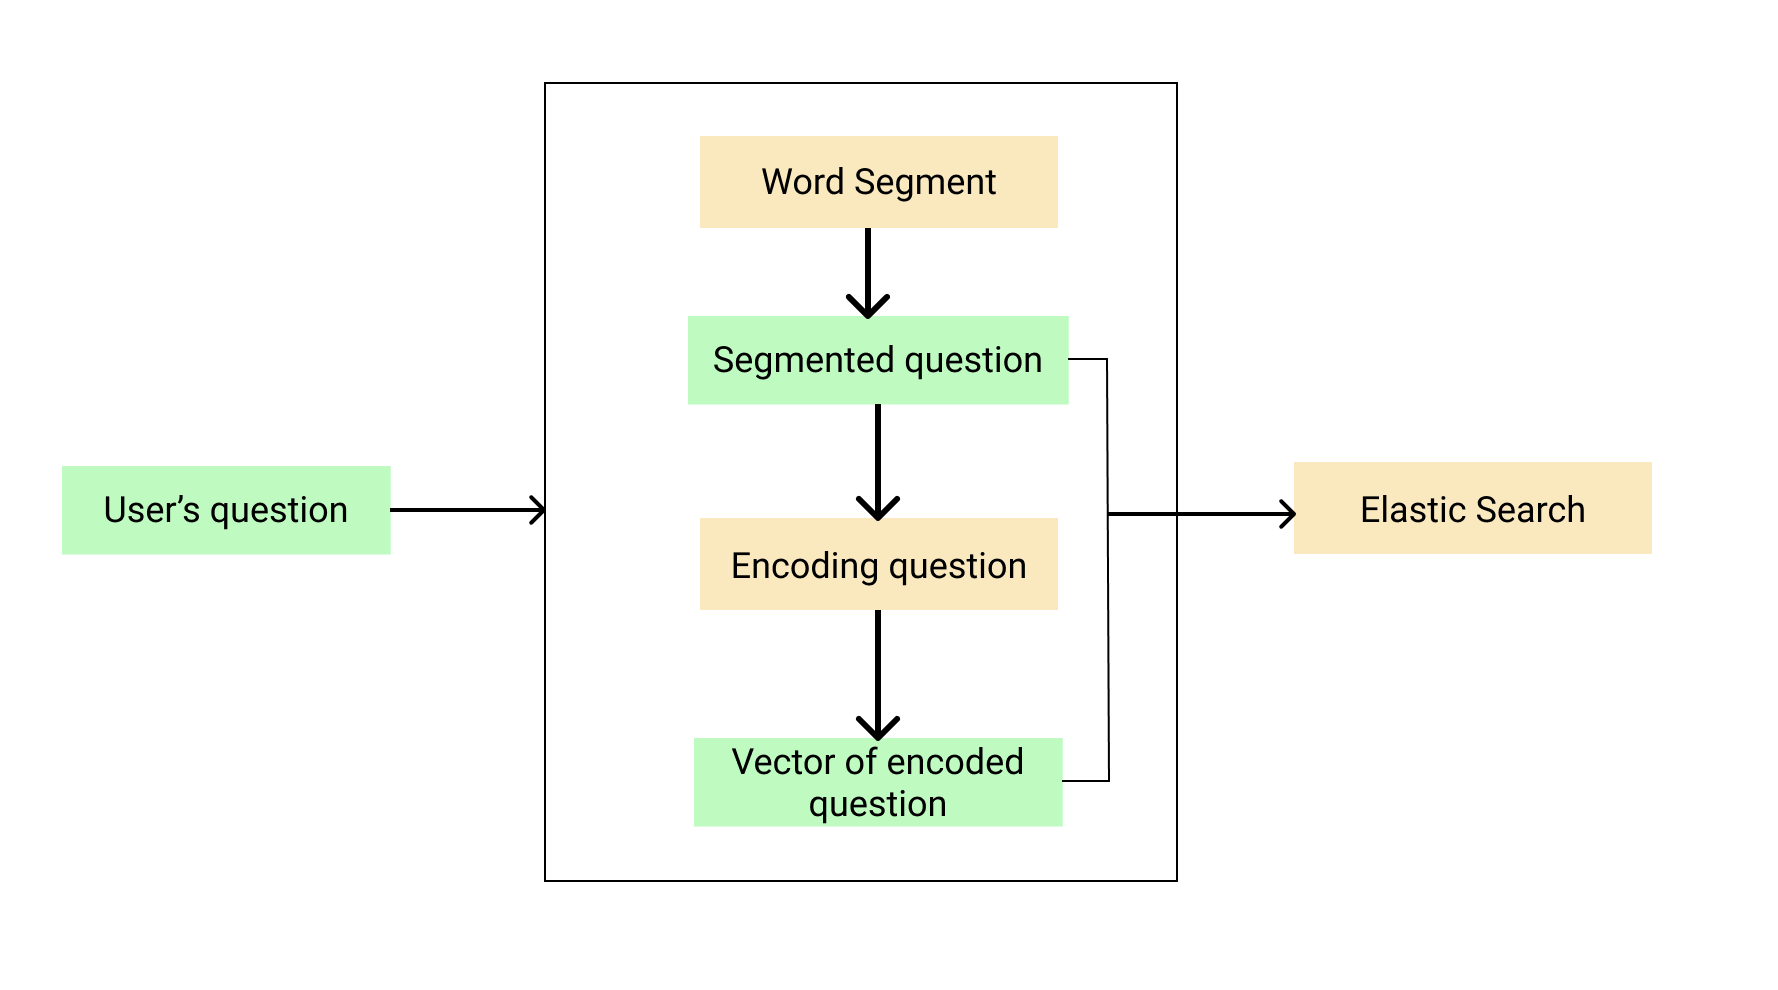
\includegraphics[width=\linewidth, height=7 cm]{images/elasticsearch_e}
\caption{Quy trình lưu dữ liệu xuống Elastic Search}
\label{fig:system2_s}
\end{figure*}

\pagebreak
\subsection{Phân loại từ trong câu hỏi}
Đầu tiên cần phải đề cập lại ở đây là có 3 cột dữ liệu đang có trong bộ dữ liệu đã được thu thập(dataset). Đó là cột câu hỏi, câu trả lời, ngày hỏi. Vì mục đích của hệ thống là hỏi đáp, đưa ra câu trả lời đúng và có mức độ liên quan gần nhất so với câu hỏi của người dùng nên đơn giản là chỉ ra được câu hỏi của người dùng nhập vào có bao nhiêu phần trăm là đồng nghĩa với câu hỏi có trong cơ sở dữ liệu. Vậy nên việc mã hoá dữ liệu cần phải làm là ở trên cột câu hỏi của dataset và câu hỏi của người dùng nhập vào từ giao diện website.

Trước khi mã hoá từ thì cần phải thực hiện một bước trước tiên đó là tách từ. Lý do cần phải thực hiện bước này trước tiên là vì tiếng việt là một ngôn ngữ không đơn giản, tiếng việt có tồn tại bên trong là các \textbf{từ ghép}. Vậy nên, nếu không thực hiện bước này trước tiên thì sẽ tạo ra một sự sai lệch về ngữ nghĩa trong khi mã hoá câu.

Ở đây thì nhóm sẽ thực hiện tách từ trong cột dữ liệu "Question" bằng PyVI như sau:

\begin{lstlisting}
	titles = [tokenize(doc["question"]) for doc in docs]
\end{lstlisting}

Dòng code này sẽ thực hiện công việc tách các từ ra, phân loại các từ đơn và từ ghép với nhau bằng dấu "$\_$".

\begin{figure*}[htp]
	\centering
	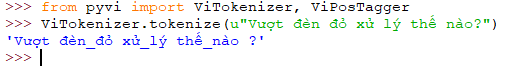
\includegraphics[scale=0.8]{images/tokenize}
	\caption{Tokenize một câu hỏi từ dataset}
	\label{fig:tokenize}
\end{figure*}

Khi thực hiện tách từ xong, biến dữ liệu \textbf{\textit{titles}} kiểu \textbf{str} sẽ lưu giữ tất cả các câu đã được tách từ. Theo như sơ đồ quy trình thì đây là thực hiện xong được bước Word Segment và được kết quả titles là Segmented question.
\pagebreak
\subsection{Mã hoá dữ liệu từ dataset}

Kết quả sau giai đoạn phân tách sẽ được hệ thống mã hóa, chuyển hóa thành các vector biểu diễn thông tin. Tại đây, nhóm áp dụng mô hình SimCSE cho tiếng Việt\cite{SimCSE_VNMESE} được phát triển dựa trên mô hình đào tạo sẵn là PhoBERT, với mục đích mã hóa, chuyển hóa thành các vector có thể biểu diễn đầy đủ ngữ nghĩa của từ của câu hỏi người dùng.\\

\begin{figure*}[htp]
	\centering
	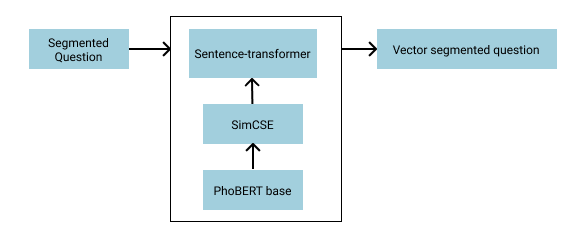
\includegraphics[scale=0.8]{images/encoding_graph}
	\caption{Quy trình thực hiện Encoding question}
\end{figure*}

Tại đây, dữ liệu đầu vào sẽ được chức năng Mã hóa thực hiện như sau:
\begin{itemize}
	\item Dữ liệu đầu vào sẽ được tính toán mã hóa dựa trên các từ, vị trí câu, vị trí từ trong câu với độ dài câu tối đa trong Position Embedding – mã hóa vị trí từ, là 512 tokens. 
	\item Token đầu tiên trong mỗi chuỗi đều có giá trị là [CLS], đại diện cho cả câu trong tác vụ phân loại. Token [SEP] dùng để phân biệt các câu với nhau.
	
	\begin{figure*}[htp]
		\centering
		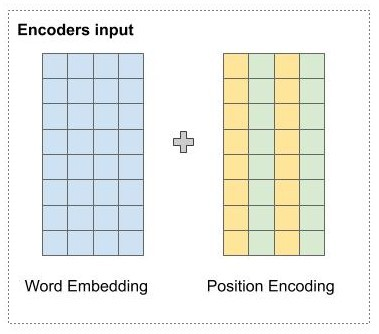
\includegraphics{images/position}
		\caption{Encoders Input}
		\label{fig:position}
	\end{figure*}
	\item Position Embedding – mã hóa vị trí từ trong câu: kiến trúc của BERT dựa trên kiến trúc của Transformers cho nên việc mã hóa vị trí từ trong câu cũng khá giống nhau. Vì Transformers có khả năng xử lý các từ song song nhưng nếu chỉ xử lý với mô hình Word Embedding sẽ không thể nào mô hình biết được vị trí của các từ để có thể hiểu ngữ nghĩa của câu. Vì vậy, cơ chế mã hóa vị trí từ trong câu xuất hiện để giải quyết vấn đề này bằng cách đưa thông tin vị trí của từ vào trong vector đại diện đầu vào.\\
\end{itemize}

Đối với việc mã hóa vị trí từ trong câu, PhoBERT hay BERT đều sử dụng công thức sau để tính toán vị trí\cite{TransformerModel}:

(PE)$_(pos,2i)$ = $\sin(pos/10000^{(2i/d_{model})})$

(PE)$_(pos,2i+1)$=$\cos(pos/10000^{(2i/d_{model})})$

Trong đó, pos là vị trí của từ trong câu, PE là giá trị phần tử thứ i trong ma trận Word Embedding có độ dài d$_{model}$.

Với việc mã hóa thành vector, SimCSE hay PhoBERT hay BERT đều dựa trên Transformers, sử dụng một cơ chế chung, cơ chế Attention., cho phép các từ khi được mã hóa sử dụng thông tin các từ liên quan đến nó.

Với mỗi từ, sẽ có ba vector tương ứng là Query, Key và Value. Các vector này được tính toán dựa trên ma trận Word Embedding.

Trong đó:
\begin{itemize}
	\item Query: vector đại diện, chứa thông tin của từ được tìm kiếm.
	\item Key: vector chứa thông tin của các từ được so sánh với vector Query.
	\item Value: vector chứa thông tin về nội dung, ý nghĩa của các từ trong vector Key.\\
\end{itemize}
Các bước tính toán attention vector có thể tóm lại bằng ba bước:

\begin{itemize}
	\item Bước 1: Tính ma trận Query, Key và Value dựa trên ma trận dữ liệu đầu vào là Word Embedding cộng với ma trận Position Embedding, tạo ra ba ma trận trọng số tương ứng với ba vector và nhân với ma trận dữ liệu đầu vào.
	\item Bước 2: Attetnion Score hay còn gọi là điểm tương quan hay trọng số, được tính bằng cách nhân hai ma trận Query và Key để so sánh mối liên hệ giữa các vector, cho ra được sự tương quan giữa chúng. Sau đó, dùng hàm Softmax để chuẩn hóa kết quả về đoạn [0-1] với ý nghĩa 1 là vector Query tương quan với vector Key, 0 là không có sự tương quan nào giữa chúng.
	\item Bước 3: Tính trọng số kết quả đầu ra bằng cách nhân ma trận kết quả Attention Score với ma trận Value để biểu diễn được thông tin của từ. \\	
\end{itemize}

\begin{figure*}[htp]
	\centering
	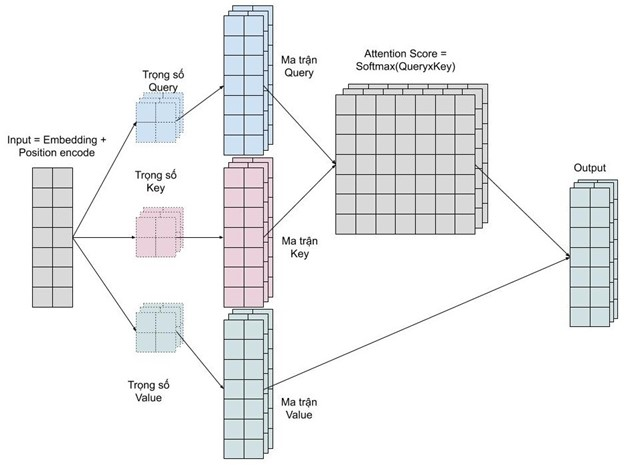
\includegraphics{images/matrix_encode}
	\caption{Ma trân mã hoá dữ liệu của BERT\cite{transformer}}
\end{figure*}

Trong thành phần Encoder của Transformers hay của BERT, thành phần Encoder bao gồm hai phần chính là Multi-Head Attention và Feedforward Network. Về bản chất, Multi-Head Attention là bao gồm nhiều lớp Self-Attention với cơ chế Attention đã được trình bày ở trên. Với mỗi Self-Attention sẽ cho ra được một mẫu kết quả khác nhau, nên việc sử dụng nhiều lớp Self-Attention sẽ giúp cho mô hình BERT cho ra kết quả chuẩn, có độ chính xác cao. Nó cho phép mô hình học được sự tương quan của từ dựa trên:
\begin{itemize}
	\item Từ kế trước của một từ
	\item Từ kế sau của một từ
	\item Những từ liên quan, tương đồng với một từ.
	
\end{itemize}

Lấy ví dụ người dùng nhập câu hỏi "Vượt đèn đỏ thì xử lý thế nào", sau khi phân tách thành các từ khóa "Vượt", "đèn\_đỏ", "xử\_lý", "thế\_nào", đưa vào mã hóa chuyển thành vector sẽ được nhận được ma trận vector của câu sau mã hóa với độ dài 768 tokens:

\begin{lstlisting}
[ 	1.9085e-01,  9.2255e-02, -8.8180e-02,  2.4886e-01, -1.8775e-02,
	...
	1.8846e-01,  3.8965e-02, 5.0931e-02,  6.2369e-02, -2.3854e-01]]
\end{lstlisting}

Cuối cùng, thực hiện xong quy trình mã hoá thì ta nhận được kết quả là Vector of encoded question như trên mô hình quy trình lưu dữ liệu xuống Elastic Search ở trên.

\subsection{Lưu dữ liệu đã mã hoá vào Elastic Search}

Sau khi có được 2 cột dữ liệu cần thiết là Segmented Question và Vector of encoded question, ta tiến hành thêm dữ liệu vào trong Elastic Search.

Đầu tiên, những giữ liệu chúng ta cần phải lưu lại trong Elastic Search cần có là:

\begin{table}[htp]
	\centering
	\begin{tabular}{|l|l|}
		\hline
		Tên thuộc tính & Kiểu dữ liệu \\ \hline
		ID             & text         \\ \hline
		Title          & text         \\ \hline
		Question       & text         \\ \hline
		Answer         & text         \\ \hline
		Title\_vector  & text         \\ \hline
	\end{tabular}
	\caption{Bảng kiểu dữ liệu thêm vào cơ sở dữ liệu}
	\label{tab:data-type-table}
\end{table}

\pagebreak
Để định danh các kiểu dữ liệu này trước khi lưu xuống cơ sở dữ liệu, ta cần một file để định danh cấu trúc của dữ liệu như sau:

\lstinputlisting[breaklines]{SourceCode/index.json}

Sau khi đã có file định danh cấu trúc cho dữ liệu, ta sử dụng thư viện Elasticsearch để bulk dữ liệu từ các biến lưu trữ thông tin về tách từ câu hỏi, vector tách từ câu hỏi vào trong Elastic Search.

Lý do để phải thêm 2 cột dữ liệu mới là vì trong khi tính toán độ tương đồng về ngữ nghĩa của câu thì cần phải so sánh với nhau ở dạng vector với nhau, từ đó mà đưa ra được kết quả chính xác hơn. 
\pagebreak
\subsection	{Kết quả}
Sau khi thêm dữ liệu thành công vào trong Elastic Search, để kiểm tra thông tin lưu trong Elastic Search thì ta thực hiện mở URL sau trên trình duyệt:

\begin{lstlisting}
	http://localhost:9200/demo_simcsejson/_search?pretty=true
\end{lstlisting}

Sau khi truy cập vào URL trên, Elastic Search sẽ trả về dữ liệu được lưu trữ trong có dạng như sau:

\begin{figure*}[htp]
\centering
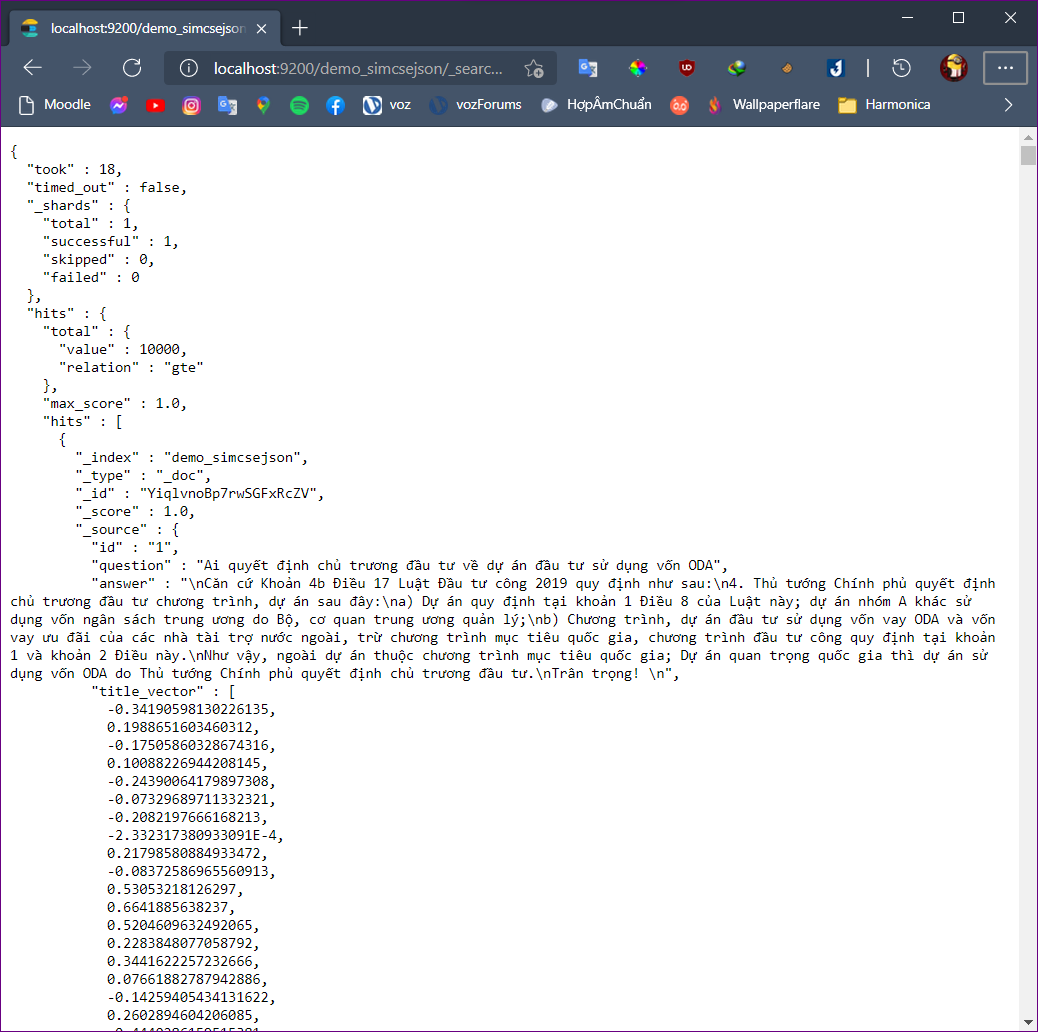
\includegraphics[width=\linewidth]{images/elastic_search_result}
\end{figure*}
\pagebreak
\section{Xử lý câu hỏi từ người dùng}
Ở mục này, câu hỏi sẽ được người dùng nhập vào trong hệ thống và được hệ thống xử lý tìm kiếm bằng cách so sánh mức độ tương đồng về ngữ nghĩa thông qua việc mã hoá câu hỏi của người dùng nhập vào thành vector câu hỏi rồi so sánh với các vector câu hỏi có trong cơ sở dữ liệu.

\begin{figure*}[htp]
\centering
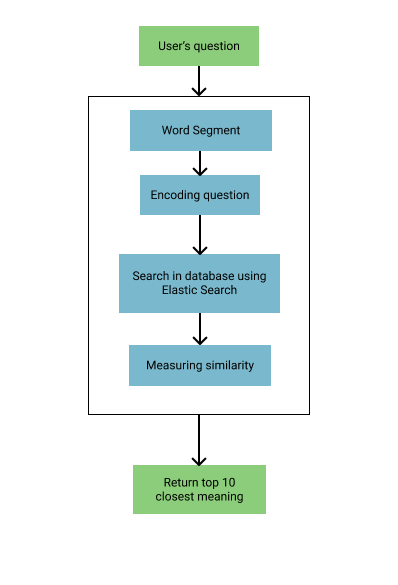
\includegraphics[width=12 cm]{images/asking}
\caption{Quy trình xử lý câu hỏi từ người dùng}
\label{fig:asking}
\end{figure*}
\pagebreak
Câu hỏi của người dùng sau khi nhập vào từ giao diện website sẽ được gửi từ web server đến phía Back-end của hệ thống. Khi nhận được dữ liệu câu hỏi, hệ thống sẽ bắt đầu thực hiện xử lý câu hỏi của người dùng theo từng bước là:
\begin{itemize}
	\item Tách từ trong câu
	\item Mã hoá câu đã được tách từ
	\item Tìm kiếm trong cơ sở dữ liệu vector giống với vector câu hỏi nhất
	\item So sánh mức độ tương đồng với câu hỏi
	\item Trả về những câu hỏi có mức độ tương đồng ngữ nghĩa với câu hỏi của người dùng cao nhất
\end{itemize}
\subsection{Tính toán mức độ tương đồng ngữ nghĩa giữa các câu}
Ở mục này, nhóm sẽ giải quyết bài toán được đặt ra từ trước để có thể tiến hành hoàn thành hệ thống là bài toán tính mức độ tương đồng ngữ nghĩa giữa các câu.

Sau quá trình tìm hiểu các phương pháp được giới thiệu để tính toán được mức độ tương đồng giữa các vector với nhau, các phương pháp đều quy về một hướng đó là so sánh khoảng các giữa các vector với nhau. Có 3 phương pháp so sánh vector với nhau mà được Google giới thiệu trong khoá học\cite{MeasureSimilarityGoogle} là:

\begin{itemize}
	\item Euclidean distance: Khoảng cách Euclide giữa hai vector
	\item Cosine: Góc giữa hai vector
	\item Dot Product: Tích vô hướng giữa hai vector
\end{itemize}

Xét riêng tích vô hướng giữa hai vector và góc giữa hai vector, chúng sẽ là giống nhau khi độ dài hai vector cùng bằng nhau và bằng 1. Nhưng nếu độ dài của hai vector không bằng 1 thì việc tính toán bằng tích vô hướng giữa các vector sẽ trở nên phức tạp hơn so với khi sử dụng góc giữa các vector. Vậy nên nếu phải chọn phương pháp nào giữa tích vô hướng và góc giữa các vector thì sử dụng góc giữa các vector sẽ là sự lựa chọn tốt hơn.

Bên cạnh đó, việc sử dụng khoảng cách Euclide trong không gian nhiều chiều sẽ được tính theo công thức là:
\begin{figure*}[htp]
\centering
$d\left( p,q\right)   = \sqrt {\sum _{i=1}^{n}  \left( q_{i}-p_{i}\right)^2 }$
\end{figure*}

Nhìn vào công thức tính góc giữa các vector là:

\begin{figure*}[htp]
	\centering
$\text{similarity}=\cos(\theta )={\mathbf {A} \cdot \mathbf {B}  \over \|\mathbf {A} \|\|\mathbf {B} \|}={\frac {\sum \limits _{i=1}^{n}{A_{i}B_{i}}}{{\sqrt {\sum \limits _{i=1}^{n}{A_{i}^{2}}}}{\sqrt {\sum \limits _{i=1}^{n}{B_{i}^{2}}}}}} $
\end{figure*}

Nếu xét trên không gian nhiều chiều, ta sẽ thấy được rằng công thức giữa Euclide distance và Cosine Distance cũng sẽ đưa về một điểm chung đó là góc giữa hai vector. Vậy nên, sử dụng Cosine Distance sẽ là sự lựa chọn thích hợp trong trường hợp này. Ngoài ra, khi sử dụng chung với Elastic Search thì sẽ được Elastic Search hỗ trợ hàm được xây dựng sẵn trong việc tính toán.

Với Ai và Bi là thành phần của vector A và B tương ứng. Giá trị của cosine luôn nằm trong đoạn [-1,1]:
\begin{itemize}
	\item Giá trị cosine bằng 1, hai vector trùng nhau, suy ra, A và B giống nhau.
	\item Giá trị cosine càng tiến về -1, nghĩa là A và B khác nhau.
\end{itemize}

Như vây, nếu giá trị cosine giữa hai vector càng tiến về 1, hai vector càng có sự tương đồng với nhau. Áp dụng vào hệ thống, ta suy ra được, nếu giá trị cosine giữa vector đại diện câu hỏi của người dùng và vector đại diện câu hỏi trong bộ dữ liệu càng gần 1, thì nội dung hai câu hỏi càng tương đồng.

Nhóm em đã tiến hành tìm kiếm sự tương đồng giữa vector đại diện câu hỏi người dùng và vector đại diện câu hỏi trong bộ dữ liệu bằng cách truyền vector đại diện câu hỏi người dùng vào Elastic Search, tính độ tương đồng Cosine Similarity nhờ vào hàm chức năng của Elastic Search. Cosine Similarity trên Elastic Search sau khi tính toán sẽ cộng thêm 1 để tránh giá trị âm, như vậy giá trị cosine nằm trong [1,2]. Về mặt ý nghĩa không khác gì giá trị cosine nằm trong [-1,1]. Chúng em thu được một số kết quả như sau:


\subsection {Trả về kết quả sau khi so sánh}
Vì Elastic Search có hỗ trợ trong việc tính toán Cosine Distance, vậy nên trong khi tìm kiếm dữ liệu bằng Elastic Search, ngoài điều việc tìm kiếm các tách từ giống nhau thì ta chèn thêm một điều kiện nữa là có Cosine Distance nhỏ nhất.

Sau đây là đoạn script dùng để search dữ liệu trong Elastic Search:
\begin{lstlisting}
 	"script_score": {
		"query": {
			"match_all": {}
		},
		"script": {
			"source": "cosineSimilarity(params.query_vector, 'title_vector') + 1.0",
			"params": {"query_vector": query_vector}
		}
	}
\end{lstlisting}

Khi nhìn vào đoạn script trên, query\_vector là câu hỏi của người dùng nhập vào được tách từ(Word Segment) và cosineSimilarity là điều kiện search khi ánh xạ qua so với Query search của cơ sở dữ liệu quan hệ.
 

Câu hỏi của người dùng: “Vượt đèn đỏ thì xử lý thế nào”.
\begin{itemize}
	\item Vector đại diện cho “Mức phạt hành vi vượt đèn đỏ” cho giá trị độ tương đồng bằng 1.8454137.
	\item Vector đại diện cho “Phạt bao nhiêu nếu ô tô vượt đèn đỏ” cho giá trị độ tương đồng bằng 1.7503384
	\item Vector đại diện cho “Hành vi điều khiển xe máy mà vượt đèn đỏ sẽ bị xử phạt bao nhiêu” cho giá trị độ tương đồng bằng 1.7825083.
	\item Vector đại diện cho “Sử dụng biển quảng cáo che mất đèn đỏ giao thông xử phạt thế nào” cho giá trị độ tương đồng 1.7325894.
\end{itemize}

Sau khi đã lấy ra được tập câu hỏi và trả lời thoả mãn được yêu cầu của hệ thống thì cần phải trả về kết quả ra để phía web server có thể lấy được kết quả trả về để gửi lại phía bên phía Front-end, hiển thị kết quả cho người dùng.
